
\section{Conceitos}

\begin{frame}{Conceitos - BRDFs}

As BRDFs calculam a proporção entre a energia luminosa que atinge um ponto na superfície e como essa energia é:
    \begin{itemize}
        \item \textbf{Refletida}
        \item \textbf{Transmitida}
        \item \textbf{Absorvida}
    \end{itemize}
    \begin{figure}[H]
        \begin{center}
            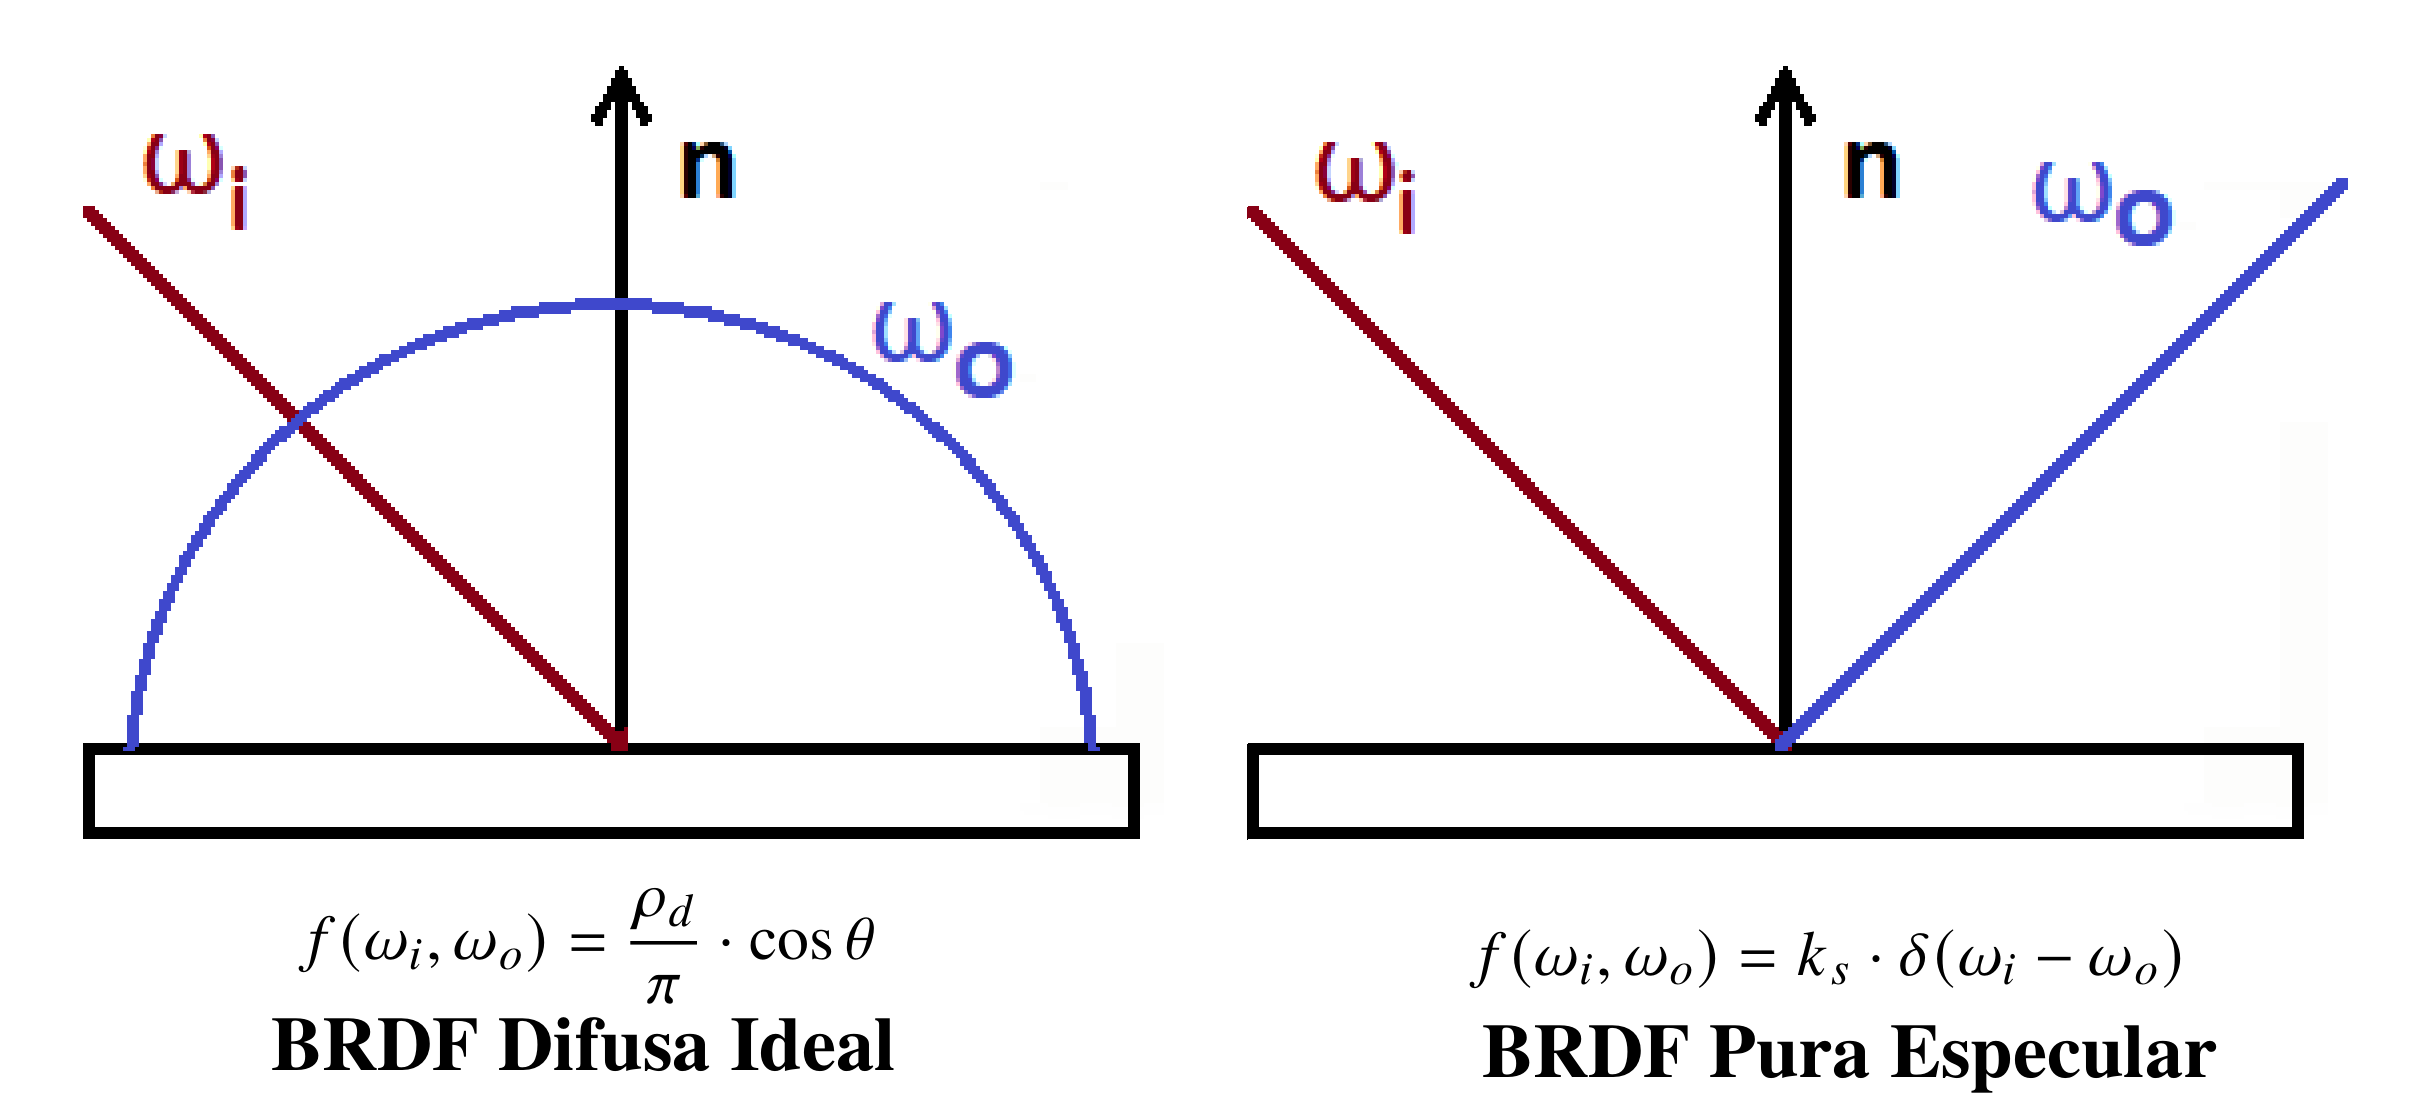
\includegraphics[width=0.65\textwidth]{./Imagens/difusa-e-specular.png}
        \end{center}
    \end{figure}
\end{frame}


\begin{frame}{Equação de Renderização}
Um renderizador estima a ``quantidade'' luz $L_o$ que sai de um ponto em uma direção ${\omega}_o$ usando a equação de renderização (\cite{rendering_equation}). Nela, a BRDF é encontrada:

    \begin{columns}
        \column{0.6\textwidth}
\begin{equation}\label{eq-rendering-equation}
\begin{aligned}
  &L_o(p, {\omega}_o) = L_e(p, {\omega}_o) +
\int_{H^2}f(p, {\omega}_i, {\omega}_o){L_i(p,{\omega}_i)\cos(\theta_i)d{\omega}_i}\\
    &L_o \text{ é radiância de saída}\\
    &L_e \text{ é radiância emitida pela superfície \tiny{(i.e. fonte de luz)}}\\
    &L_i \text{ é radiância incidente na superfície}\\
    &{\omega}_i \text{ é a direção do raio incidente}\\
    &{\omega}_o \text{ é a direção do raio refletido}\\
    % &H^2 \text{ são todas as direções no hemisfério no ponto $p$}\\
    % &\theta_i \text{ ângulo entre direção incidente e a normal da superfície}\\
    &f \text{ função de refletância}\\
\end{aligned}
\end{equation}
\column{0.4\textwidth}
    \begin{figure}[H]
        \caption{\cite{MicrofacetBRDF}}
        \vspace{2cm}
        \hspace{2cm}
        \begin{center}
            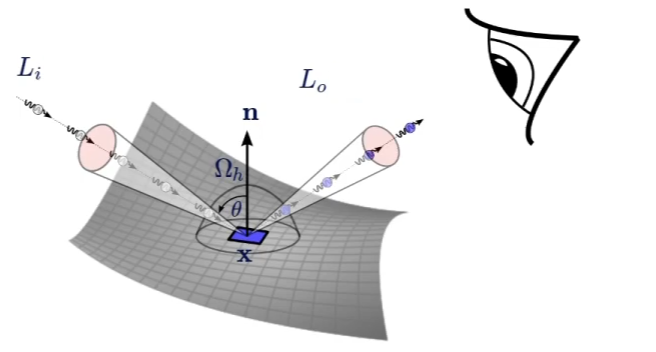
\includegraphics[width=0.65\textwidth]{./Imagens/Li-Lo.png}
        \end{center}
    \end{figure}
    \end{columns}
\end{frame}



% SLIDE 2
\begin{frame}{\textit{Pipeline} de GPU}
    Etapas Principais:
    \begin{enumerate}
        \item \textbf{\textit{Shader} de Vértice}: Processa e transforma vértices.
        \item \textbf{Rasterização}: Gera fragmentos a partir de primitivas.
        \item \textbf{\textit{Shader} de Fragmento}: Determina a cor final dos fragmentos.
    \end{enumerate}

    Fluxo de dados são:  CPU $\to$ GPU $\to$ \textit{Shaders} $\to$ Imagem final.
    \begin{figure}[H]
        % \centering
        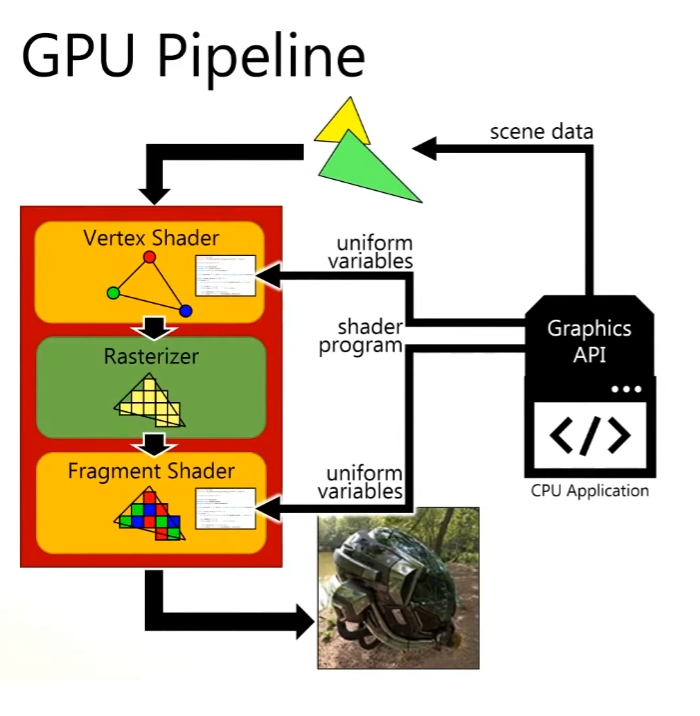
\includegraphics[scale=0.25]{./Imagens/gpu_pipeline.png}
        % \caption{\small Representação do \textit{pipeline} de GPU.}
    \end{figure}
\end{frame}

% SLIDE 3
\begin{frame}[fragile]{\textit{Shader} de Vértice}
    \begin{itemize}
        \item Aplicação de transformações (ex.: rotação, projeção).
        \item Transmissão de dados (ex.: normais) ao \textit{shader} de fragmento.
    \end{itemize}

    \begin{clang}
#version 330 core
layout(location = 0) in vec3 inPosition;
layout(location = 1) in vec3 inNormal;

uniform mat4 modelViewProjection;

out vec3 fragNormal;

void main() {
    vec3 manipulatedPosition = inPosition + (sin(gl_VertexID * 0.1) * 0.1);
    fragNormal = inNormal;
    gl_Position = modelViewProjection * vec4(manipulatedPosition, 1.0);
}
    \end{clang}
\end{frame}

% SLIDE 4
\begin{frame}{\textit{Shader} de Fragmento}
    Nesse \textit{shader} é onde a cor final é calculada. Roda paralelamente 1 vez para cada ``pixel''.
    \begin{figure}[H]
        \centering
        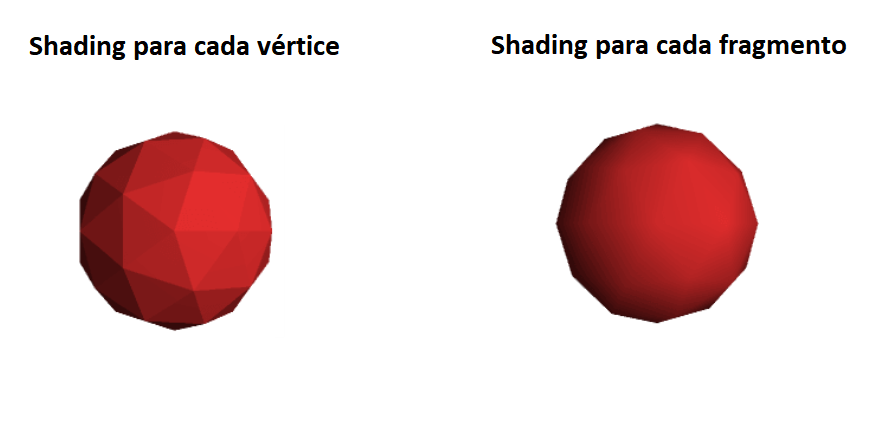
\includegraphics[scale=0.5]{./Imagens/per_vertex_per_frag.png}
        \caption{\small Diferença entre \textit{shading} por vértice e por fragmento.}
    \end{figure}
\end{frame}

% \begin{frame}{Shaders e implementação}
%     \begin{itemize}
%         \item Na renderização, BRDFs são implementadas por \textit{shaders}, programas especializados executados na GPU.
%         \item APIs gráficas permitem programar esses shaders em diferentes etapas do processo de renderização ( OpenGL).
%         \item Com os shaders, cada objeto renderizado pode ter sua aparência configurada por meio de códigos que implementam BRDFs específicas.
%     \end{itemize}
% \end{frame}

\begin{frame}{Compilação: Visão Geral}
    Compilador $C: L_1 \rightarrow L_2$ mapeia programa de $L_1$ para $L_2$ preservando semântica\footnote{\tiny{Mantém mesmo significado algorítmico}}.

    \begin{enumerate}

        \item \textbf{Análise Léxica (Lexing):}
              \begin{itemize}
                  \item Divide entrada em tokens (palavras-chave, identificadores)
                  \item Reconhecível por máquinas de estado
              \end{itemize}
        \item \textbf{Análise Sintática (Parsing):}
              \begin{itemize}
                  \item Constrói árvore sintática baseado nas regras de produção
              \end{itemize}
        \item \textbf{Verificação Semântica:}
              \begin{itemize}
                  \item Garante consistência de tipos, assinatura de funções, significado dos símbolos, etc.
                  \item No nosso caso, previne erros na modelagem da BRDF
              \end{itemize}
        \item \textbf{Emissão de Código:}
              \begin{itemize}
                  \item Gera código na linguagem alvo
              \end{itemize}
    \end{enumerate}
\end{frame}

